\documentclass[UTF8]{pkuthss}

\usepackage[backend = biber, style = caspervector, utf8, sorting = ecnty]{biblatex}
\usepackage{amssymb}
\usepackage{amsmath}
\usepackage{graphicx}
\usepackage{deluxetable}
\usepackage{color}

\setlength{\bibitemsep}{3bp}
\renewcommand*{\bibfont}{\zihao{5}\linespread{1.27}\selectfont}

\pkuthssinfo{
	cthesisname = {硕士研究生学位论文}, ethesisname = {Master Thesis},
	ctitle      = {基于近场动力学理论的弹塑性材料碎裂仿真},
    etitle      = {Peridynamics-Based Fracture Animation for Elastoplastic Solids},
	cauthor     = {陈伟},
	eauthor     = {Wei Chen},
	studentid   = {1501214372},
	date        = {二〇一八\ 年\ 六\ 月},
	school      = {信息科学技术学院},
	cmajor      = {计算机软件与理论},
    emajor      = {Computer Software and Theory},
	direction   = {计算机图形学},
	cmentor     = {李胜\ 副教授},
    ementor     = {Sheng Li},
	ckeywords   = {近场动力学,碎裂,弹塑性, 仿真},
    ekeywords   = {peridynamics, fracture, elastoplasticity, animation}
}

\addbibresource{thesis.bib}


\def\pkuthssffaq{%
	\emph{\textcolor{red}{pkuthss 文档模版最常见问题:}}

	\texttt{\string\cite}、\texttt{\string\parencite} %
	和 \texttt{\string\supercite} 三个命令分别产生%
	未格式化的、带方括号的和上标且带方括号的引用标记:%
	\cite{test-en},\parencite{test-zh}、\supercite{test-en, test-zh}。

	若要避免章末空白页,请在调用 pkuthss 文档类时加入 \texttt{openany} 选项。

	如果编译时不出参考文献,
	请参考 \texttt{texdoc pkuthss}“问题及其解决”一章
	“其它可能存在的问题”一节中关于 biber 的说明。
}

\begin{document}

    \newcommand{\xii}{\textbf{x}_i}
\newcommand{\xj}{\textbf{x}_j}
\newcommand{\vi}{\textbf{v}_i}
\newcommand{\vj}{\textbf{v}_j}
\newcommand{\fin}{\textbf{f}_i^{int}}
\newcommand{\fex}{\textbf{f}_i^{ext}}

\newcommand{\X}{\textbf{X}}
\newcommand{\Y}{\textbf{Y}}
\newcommand{\Z}{\textbf{Z}}
\newcommand{\F}{\textbf{F}}
\newcommand{\E}{\textbf{E}}

\newcommand{\mb}[1]{\mathbf{#1}}

\newcommand{\bfT}{\textbf{T}}
\newcommand{\bft}{\textbf{t}}
\newcommand{\bfu}{\textbf{u}}
\newcommand{\bfx}{\textbf{x}}
\newcommand{\bff}{\textbf{f}}
\newcommand{\bfv}{\textbf{v}}
\newcommand{\bfy}{\textbf{y}}
\newcommand{\bfui}{\textbf{u}_{(i)}}
\newcommand{\bfvi}{\textbf{v}_{(i)}}
\newcommand{\bffi}{\textbf{f}_{(i)}}
\newcommand{\bfyi}{\textbf{y}_{(i)}}
\newcommand{\bfuj}{\textbf{u}_{(j)}}
\newcommand{\bfxi}{\textbf{x}_{(i)}}
\newcommand{\bfxj}{\textbf{x}_{(j)}}
\newcommand{\bfyj}{\textbf{y}_{(j)}}
\newcommand{\bfvj}{\textbf{v}_{(j)}}
\newcommand{\bfxl}{\textbf{x}_{(l)}}
\newcommand{\bfyl}{\textbf{y}_{(l)}}
\newcommand{\bfuk}{\textbf{u}_{(k)}}
\newcommand{\bfxk}{\textbf{x}_{(k)}}
\newcommand{\bfyk}{\textbf{y}_{(k)}}
\newcommand{\wij}{\omega_{(i)(j)}}
\newcommand{\wkj}{\omega_{(k)(j)}}
\newcommand{\wkl}{\omega_{(k)(l)}}
\newcommand{\skj}{s_{(k)(j)}}
\newcommand{\skl}{s_{(k)(l)}}
\newcommand{\fkj}{\textbf{f}_{(k)(j)}}
\newcommand{\tkj}{\textbf{t}_{(k)(j)}}
\newcommand{\tjk}{\textbf{t}_{(j)(k)}}
\newcommand{\thetai}{\theta_{(i)}}
\newcommand{\thetak}{\theta_{(k)}}

%\newcommand{\mycite}[2]{\textcolor{blue}{(#1 et al. #2)\parencite{#1#2}}}
%\newcommand{\myciteTwo}[3]{\textcolor{blue}{(#1 et al. #2\parencite{#1#2},#3\parencite{#1#3})}}
%\newcommand{\myciteThree}[4]{\textcolor{blue}{(#1 et al. #2\parencite{#1#2},#3\parencite{#1#3},#4\parencite{#1#4})}}

\newcommand{\mycite}[2]{\textcolor{blue}{(#1 et al. #2)\supercite{#1#2}}}
\newcommand{\myciteTwo}[3]{\textcolor{blue}{(#1 et al. #2\supercite{#1#2},#3\supercite{#1#3})}}
\newcommand{\myciteThree}[4]{\textcolor{blue}{(#1 et al. #2\supercite{#1#2},#3\supercite{#1#3},#4\supercite{#1#4})}}

\newcommand{\fa}{${}^{\textrm{a}}$}
\newcommand{\fb}{${}^{\textrm{b}}$}



    
	\frontmatter
	\pagestyle{empty}
	\maketitle
	\cleardoublepage

	\include{chap/copyright}


	\cleardoublepage
	\pagestyle{plain}
	\setcounter{page}{0}
	\pagenumbering{Roman}

	\begin{cabstract}
在游戏、虚拟现实、电影等工业领域需求日益增长的背景下,基于物理的碎裂仿真一直是计算机图形学中的热点问题,但此问题虽愈发得到重视,却仍极具挑战,至今没有足够成熟的解决方案。碎裂仿真的难点主要在于碎裂模式本身的复杂多样性,以及仿真的稳定性、精确性、和仿真效率。本文基于近场动力学理论,主要针对弹塑性材料的形变和碎裂行为,提出了一种新的无网格动力学仿真框架。

本文所阐述的近场动力学模型能够逼真地对弹塑性材料的形变行为进行表达,通过在实验上多样化材料的属性,然后和传统的 FEM 方法进行充分的对比,结果表明其在效果上能够取得和 FEM 共旋线性(Corotated Linear)模型几乎一致的效果,并且更具稳定性。同时,由于近场动力学本构模型使用的是积分形式的表述,其在仿真的精确性、实现的简单性、以及算法的并行化方面相对于常见的微分形式方法也更具优势。虽然近年 FEM 方法在碎裂仿真领域同样应用广泛,但其作为一种微分方法实际上将在不连续处失去意义。因此,在大形变以及碎裂情况下,往往需要对拓扑网格进行 remeshing 操作来提高网格质量,保证仿真的稳定性,其在实现上较为复杂,计算上较为耗时并且难以并行化。通过结合近场动力学本构模型以及本文所提出的碎裂模型,本文提出的动力学框架能够较好避免这一问题,实验表明本文所提出的方法能够高逼真度地模拟可扩展性材料以及脆性材料的碎裂行为。本文还通过引入各向异性矩阵核来对本构模型进行进一步的拓展,使之可模拟材料的各向异性属性。

在几何表达方面,本工作使用四面体网格来对物体进行离散,并且提出了一种简单的嵌网格策略用于追踪材料刚性运动、形变及碎裂行为。通过此嵌网格策略,也更方便于进行后续物体间的碰撞检测和反应,以及最后的渲染输出工作。

本文是图形学领域第一次使用近场动力学理论来仿真包括弹(脆)性、塑性、碎裂、各向异性等多种现象在内的工作,所提出的方法为基于物理的动力学仿真尤其是碎裂仿真提供了一种新的思路。

\end{cabstract}

\begin{eabstract}
	Test of the English abstract.
\end{eabstract}



	\tableofcontents

	\mainmatter
	\chapter{绪言}
\label{chap1_introduction}
\section{研究背景}
随着科学技术的不断向前,人们对于工程应用中的设计可靠性和虚拟应用中的真实感体验亦在不断提出更高的要求。而物理仿真作为解决此类问题的关键技术手段,在计算机硬件的不断发展和计算能力大幅度提升的背景下,近年来得以快速跨越式发展。

所谓基于物理的仿真是指通过对物理建立能够表征物体属性的动力学模型,在计算机上以某种合适的方式进行离散数值计算,对真实世界中的物理行为进行模拟。物理仿真在计算机科学中占据重要地位,并应用于多个不同的关键领域。例如,在基础物理领域,往往通过物理仿真来寻找其中的统计规律,揭示真实世界中的物理原理。在工程和材料领域,物理仿真是探索材料性质或进行辅助验证设计的重要手段。在计算机图形学领域以及电影、游戏等工业界,物理仿真更是给用户带来高逼真度沉浸式体验的关键技术。总之,物理仿真应用具备数据密集和计算密集双重特点,其作为一项基础性技术,在电影、工程设计、游戏等产业领域应用广泛、用户众多,是国家近年来大力发展的战略性新兴领域。

碎裂仿真是物理仿真领域的一个重要分支。在日常生活中,碎裂效果(如玻璃碎裂、爆炸等)往往给人以深刻印象。而碎裂仿真便是通过对材料建立合适的动力学模型,设置材料的真实物理参数以及碎裂条件,使用基于物理的方法来对物体的断裂进行动态计算。但相对于工业界以及材料科学领域对于仿真精确性的高要求,图形学领域的应用更强调系统的稳定性和视觉效果,为提高效率,往往倾向于对模型进行一定的简化以更快的得到结果。

碎裂仿真是游戏动画、数字电影和工程仿真等领域的研究热点,其具有极大的应用价值。在电影特效领域,出于成本以及人员安全的考量,真实地拍摄爆炸等大规模碎裂场景往往不具有可行性。而通过高性能计算机进行碎裂仿真,不仅能够降低电影的制作成本,而且可以控制整个断裂或者碎裂的过程,还有利于艺术家的后期设计与制作。在游戏领域,碎裂现象的实时模拟更是交互的重要组成部分,是给予玩家真实游戏体验的关键要素。在工程领域,碎裂仿真是研究材料特性以及进行结构设计(如房屋倒塌)的重要手段。在国防领域,因为炸弹轰击而产生的爆炸效果也是碎裂的一种典型现象,对于爆炸效果的碎裂仿真将极其有助于研究武器的杀伤力,进行武器的设计。弹塑性物体的碎裂在生活中也随时可见,如橡胶材料的碎裂。手术时对人体器官的切割实际上也是一种形变体碎裂,研究在虚拟手术中的人体组织器官的交互式切割仿真,可应用于手术演示和手术人员的操作训练,起到重大辅助作用,更具有广阔的前景。

虽然近年来,碎裂仿真已经在学术界得到广泛研究。但至今为止,仍然缺乏能够在计算的效率上、计算的稳定性和可靠性上以及实现的简单性上能够支撑其工业界应用的仿真方法,更为成熟的碎裂仿真模型亟待进一步探索。本文的目的即是从近场动力学理论出发,提出了一整套用于弹塑性材料的可延展性碎裂和脆性碎裂的仿真框架,为碎裂仿真提供新的思路。

\section{相关工作综述}
\label{related_work}
近年来,在计算能力不断提升和人们对于真实度体验有更高需求的背景下,碎裂现象愈发成为虚拟游戏和电影等不同领域应用中不可或缺的一部分。碎裂仿真在工程和计算机图形学等领域已经得到广泛研究,并且在学术界提出了各式各样的算法,具体参见综述\mycite{muguercia}{2014} , \mycite{Wu}{2015}。 从已有研究成果来看,可以主要分为有网格方法和无网格方法两类。

\subsection{有网格方法}

早期的碎裂仿真工作受限于计算能力,更倾向于使用简单的建模或计算方式来进行模拟。例如\mycite{Terzopoulos}{1988}使用有限差分方法(The Finite Difference Method),\mycite{Norton}{1991}使用质点弹簧系统,\mycite{Smith}{2001}使用物质点约束系统等。

随着学术界的探索,各式各样的仿真算法也被不断提出。但到目前为止,所有基于网格的仿真法中,有限元方法(FEM)应该是应用最为广泛的。FEM 方法基于连续介质力学的分析,然后对物体所在空间进行离散化,然后对各离散点的物理状态进行仿真,以得到较为精确的结果。一般而言,物体被分解为一个四面体网格或者包含其他元素的体网格,给定一个本构模型,可以对体网格中的所有元素进行应力分析,然后将计算得到物理参数以加权的形式累加到与元素相关的几何节点上,最终形成一个全局线性方程来更新各节点的物理状态。如果施加到离散节点的应力超过阈值,则根据一定的标准以及策略将几何节点进行分裂。

\textcolor{blue}{(O'Brien et al.)\parencite{OBrien1999}}在图形学领域最先使用FEM 方法来进行脆性材料的仿真,并且取得了当时最为惊艳的效果。在随后的工作中, O'Brien et al.还进行了进一步的扩展,引入一个加法形式的塑性模型,用来对可延展性材料的碎裂行为进行模拟\textcolor{blue}{(O'Brien et al. )\parencite{OBrien2002}}。 值得注意的是,本文工作所用塑性模型同样是加法形式,并且在设计上借鉴了此工作。在传统碎裂仿真中,考虑到脆性材料一般具有极大的刚度系数,往往需要极小的时间步来保证仿真的稳定性,为缓解此问题,\textcolor{blue}{(M\"{u}ller et al. )\parencite{Muller2001}}使用了基于准静态的有限元分析方法,其基本思想是脆性材料在形变上几乎可以忽略不计,所以对于分离的物体块,直接采用刚体动力学仿真,而对于碰撞产生的碎裂问题,使用准静态有限元分析来进行判断。此外,针对游戏场景中的实时碎裂仿真,\mycite{Parker}{2009} 提出了一些非常有用的技术。

在处理碰撞检测以及渲染方面,FEM 具有较大的优势。FEM 的有效性也已经被各领域的大量工作所验证,然而,其最大挑战来源于频繁的拓扑改变操作。由于在仿真过程中,顶点的频繁分裂以及对四面体进行切割,将很有可能形成质量较差的狭长的四面体,考虑到使用的一般是一阶线性的形函数(Shape Function),这些由大形变或者切分而形成狭长的四面体将极大的影响整个仿真过程的精度和稳定性。为缓解此问题,一般需要对四面体网格进行重采样以及 remeshing 保证整个网格的质量,尽管在科研领域已经提出多种 remeshing 的方法,但往往 remeshing 操作是非常费时并且难以实现的。

早期的方法直接使用沿单元体边界分裂的方法来实现碎裂,如\mycite{Norton}{1991}, \mycite{Mazarak}{1999}, \mycite{Smith}{2001}, \textcolor{blue}{(M\"{u}ller et al.)\parencite{Muller2001}},甚至是直接使用单元体删除的办法\mycite{Forest}{2002}。上述方式在处理上比较简单方便,但碎裂产生的路径却相对受限,更为复杂的方式是允许单元的的剖分,为产生的裂纹添加更为丰富的几何细节\mycite{Andrew}{2000}, \mycite{Bielser}{2000}。允许裂纹往任意方向生长虽然在效果上更为自然逼真,但付出的代价是拓扑网格质量的下降,往往需要 remeshing 操作进行弥补\mycite{Neff}{1999}, \textcolor{blue}{(O'Brien et al. )\parencite{OBrien1999}}, \textcolor{blue}{(O'Brien et al. )\parencite{OBrien2002}}。 为避免 remeshing 操作的复杂性,\mycite{Molino}{2004}提出了使用虚节点的方式,其基本原理是当碎裂发生时,在几何表达上使用虚节点的方式将分割的四面体部分拷贝,但在物理计算上对四面体进行完全复制。这一技术由于其简便性很快被应用到其他工作,包括\mycite{Bao}{2007}, \mycite{Sifakis}{2007}, \mycite{Wang}{2015}等。 \mycite{Kaufmann}{2009}进一步使用拓展的 FEM 方法(XFEM),其关键是使用自定义的基函数来进行计算,而不是使用真实或虚拟地单元体剖分方式。

其他典型的有网格方式还包括基于模态分析(Model Analysis)的方法\mycite{Glondu}{2013},以及适用于纯粹基于几何分解来进行实时脆性碎裂仿真的方法\textcolor{blue}{(M\"{u}ller et al. )\parencite{Muller2013}}, \mycite{Schvartzman}{2014}。最近,\mycite{Zhu}{2015}和\mycite{Hahn}{2015}提出使用基于边界元的方法(Boundary Element Method)来仿真刚体的碎裂,在他们的工作中,使用表面网格来同时表示物体以及进行碎裂相关的物理计算。

\subsection{无网格方法}

无网格方法早期因拓扑表达上相对受限,在碎裂仿真领域并非主流,但由于其灵活性以及近来来在几何表示难题上面的攻克,关注度不断得到提升。其不存在FEM 中关于网格拓扑质量的问题,一般仿真只是空间中离散的粒子,而并不存在网格。典型方法包括提出使用最小二乘法MLS(Moving Least Square)的无网格框架\textcolor{blue}{(M\"{u}ller et al. )\parencite{Muller2004}}。 此后,\mycite{Pauly}{2005}提出了一整套全新的无网格框架用来对弹塑性材料的碎裂进行仿真。\mycite{Steinemann}{2009}的工作基于无网格的物理计算框架,但使用显式的表面网格来对形变体的分裂进行追踪。受脆性碎裂中的刚体动力学运动近似启发,
\mycite{Liu}{2011}使用MLPG(Meshless Local Petrov-Galerkin Method)来进行应力的分析,并取得了不错的结果。
\mycite{Stomakhin}{2013}开创性地使用物质点法(MPM)来模拟雪这种特殊形态物质的碎裂现象,效果惊艳。
\mycite{Hegemann}{2013}进一步结合物质点法和基于水平集(level set)的网格对可拓展性材料进行仿真。

从视觉效果方面,离散的粒子给渲染提出了一定的挑战,所以一般会在无网格框架下,经常嵌入一个网格以便于进行渲染。无网格方法具有较高的灵活性,如果嵌入网格并处理得当,在渲染和碰撞检测上面的问题,也能得到一定程度的弥补。但无网格方法仿真大都是针对的脆性材料,在弹塑性材料方面,对应的研究上工作仍比较缺乏。所以在现阶段,学术界仍然在努力寻求更为方便以及更具效率的无网格仿真算法。

本文所提的方法即为在近场动力学的无网格框架下,通过嵌入网格来辅助进行碰撞检测和反应以及最后的渲染输出工作,来完成弹塑性材料从形变到碎裂的完整仿真。

\section{研究成果和创新点}
本文的主要研究成果是提出并实现了一种新的基于近场动力学理论的无网格框架来进行弹塑性物体的形变和碎裂仿真,其能够克服 FEM 在拓扑网格上面存在的困难,避免 remeshing 操作所引发的效率低下和实现复杂问题。在物理动力学上,其能够较为精确仿真碎裂行为,提供物理上和视觉上可信服的结果。此外,为表达弹塑性碎裂行为的视觉效果,本文还提出一种新的简单可用的嵌网格方法。本工作所提框架易于实现,具有较强的可扩展性,并且在效率上相对于传统方法更具优势。

具体而言,本文的创新点主要在于三点:
\begin{enumerate}
  \item 基于近场动力学理论,提出一种新的基于近场动力学理论无网格仿真仿真框架。其支持包括弹塑性材料的弹性形变、塑性形变、弹塑性碎裂、脆性碎裂等多种复杂物理行为,同时能够很好地解决在 FEM 中不连续性引起的奇异值问题,避免复杂耗时的 remeshing 操作。此外,本文还对模型进行进一步扩展,使其能够支持简单的各向异性行为。
  \item 设计一种简单有效的嵌网格方法,所设计策略能够对物体的形变和碎裂行为进行追踪,能用于后续的碰撞处理以及提供高质量网格以用于渲染。本文力图所提的嵌网格方法是有效,完备的,可应用于其他无网格框架,且具有良好的扩展性。
  \item 基于 Physika 物理引擎,设计并实现相应的模型和主要算法,并对实现进行大量的实验和验证工作,和已有方法(FEM)进行充分对比。
\end{enumerate}

\section{本文组织结构}
本文主要分为六章。

第\ref{chap1_introduction}章介绍本文工作的研究背景,阐述物理仿真尤其是碎裂仿真的研究意义以及在各领域的应用需求情况。梳理关于碎裂仿真的相关工作,同时明确本文的研究问题,介绍本文的研究成果和工作的创新点。

第二章对概述性地介绍了物理仿真的基本原理,以及碎裂仿真的基本流程。并针对碎裂仿真中的三个主要要素,本构模型、碎裂模型、和离散时间积分在仿真中所扮演角色和作用,进行了较为详细的阐述。

第三章 blablabla

第四章 blablabla

第五章 blablabla

第六章 blablabla
	\chapter{碎裂仿真介绍}

\section{物理仿真之基本原理}
绝大多数物理仿真流程遵循相同的基本流程,都可以认作是牛顿第二定律 $F = Ma$ 的不同形式的体现。如图\ref{fig_physically_based_animation} 所示:
\begin{figure}[htbp!]
  \centering
  \captionsetup{justification=centering}
  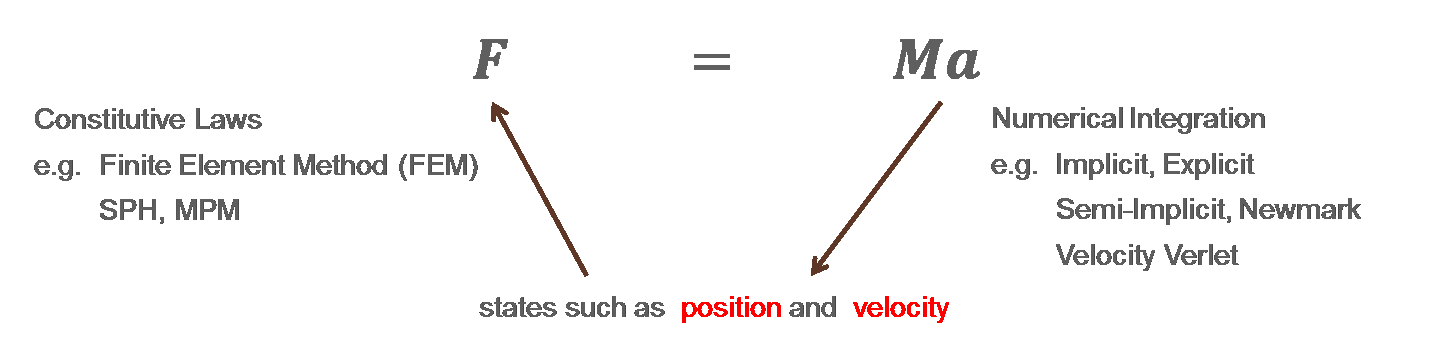
\includegraphics[width=\linewidth]{E:/Thesis-Master/chap/image/physically_based_animation}

  \caption{\label{fig_physically_based_animation}
           物理仿真动力学循环示意图。物体所受内外力、加速度、以及物体状态构成动力学循环三角。
          }
\end{figure}

在物理仿真中,需要关注三个核心的动力学要素:物体所受内外力,加速度,以及物体的状态。从物体的当前所处状态,即物体的位置和速度信息,来推导物体当前各部分所受力,所涉及的是物理仿真中最为关键的部分——动力学本构模型。通俗而言,本构模型描述的是材料的形变与动力学行为之间的关系,一般也称为内力模型。常见的本构模型包括用来描述固体运动的有限元方法(FEM)、用来描述流体运动的光滑粒子动力学(SPH)\textcolor{blue}{(M\"{u}ller et al. )\parencite{Muller2003}}、 以及适合对雪进行建模的物质点法(MPM)\mycite{Stomakhin}{2013}等。关于本构模型的一般性介绍,将呈现于章节\ref{constitutive_model}。

根据物体所受力 $F$,则可以根据牛顿第二定律直接获得物体的加速度 $a$。 而从物体所受加速度进一步推导得到物体的当前状态,所涉及到的则是离散时间积分算法。离散积分算法的作用是在给定时间步 $\Delta t$ 下,物体的状态将以何种方式进行更新。不同的离散时间积分算法对物理仿真的稳定性、精确性和效率有重大影响,本文将在\ref{numerical_method} 小节详细阐述。

可以看到,物体所受内外力、加速度、以及物体状态构成了一个动力学循环三角,并通过牛顿第二定律、本构模型、数值积分算法进行衔接。绝大部分仿真算法都是采用关键帧(key frame)的形式,因为在复杂场景中,物体的运动几乎不可能以解析的形式来表达,因此需要随着时间步而不断向前迭代,以此获得物体完整的运动状态序列。

\section{碎裂仿真之基本流程}
碎裂仿真是物体仿真的一个具体特化,但相对于传统仿真更具复杂性。其原因不仅在于碎裂模式的多样化,更在于在碎裂发生的情况下,物体本身拓扑表达的变化,导致物体单元体或节点的数量也将发生改变。常见的碎裂仿真流程如图
\ref{fig_fracture_animation_pipeline}总结:
\begin{figure}[htbp!]
  \centering
  \captionsetup{justification=centering}
  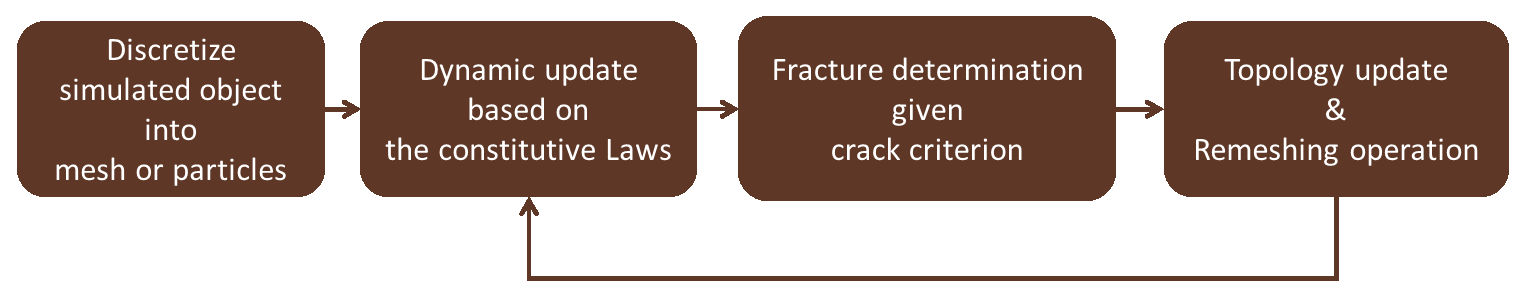
\includegraphics[width=\linewidth]{E:/Thesis-Master/chap/image/fracture_animation_pipeline}

  \caption{\label{fig_fracture_animation_pipeline}
           碎裂仿真的基本流程。主要分为四个关键步骤,分别是物体离散、动力学更新、碎裂发生判断,拓扑更新。
          }
\end{figure}

从图\ref{fig_fracture_animation_pipeline}可以看出,碎裂仿真主要包含四个步骤。

第一个步骤是在动力学仿真开始前,需要以合适的方式对物体进行离散,由于计算资源是有限的,因此不可能以无限微分的方式来对物体进行建模计算,而只能用有限的状态集表示。一般而言,离散方式和本构模型直接挂钩。对于传统基于网格的方法,如 FEM,通常将物体离散成四面体或六面体体网格,对于薄壳体则离散成三角面片网格\mycite{Pfaff}{2014}。而对于无网格方法,则通过粒子集合来表示物体\mycite{Pauly}{2005}。

第二个步骤是在物体已知状态下,通过动力学本构模型和数值积分算法来对物体的状态进行更新,这一步骤是所有物理仿真所必须的。

第三个步骤和第四个步骤是根据给定的碎裂标准和阈值判断物体中的某些节点是否应该发生碎裂,碎裂模型一般建立在已有的本构模型之上,本文将在\ref{fracture_model}进行一般性介绍。如果判断物体部分节点发生碎裂,则往往需要对拓扑进行更新。对于有网格方法,在必要情况下,还需要对拓扑网格进行 remeshing 操作以对网格进行精化。在拓扑更新完之后,将进入下一个循环的动力学更新。关于本文工作所用的碎裂模型和拓扑更新方式,将分别在第三章和第四章进行阐述。

\section{本构模型泛述}
\label{constitutive_model}
在图形学领域及工程材料领域,一般研究的是物质的宏观运动。但实际上物质都是由大量分子组成的,分子间的真空区尺度远大于分子本身,并且每个分子在无休止的做不规则运动,相互间经常碰撞,交换着动量和能量。因此物质的微观结构和运动无论在时间上还是空间上都充满着不均匀性、离散性和随机性。而另一方面人们用仪器测量或者用肉眼观察到的物质宏观结构和运动却又明显呈现出均匀性、连续性和确定性。这两种特性如此之不同却又和谐统一地表现于物质之中。研究物体的宏观运动存在两种不同的途径,一种是基于统计物理的方法,其直接从分子和原子的运动出发,采用统计平均的方法建立宏观物理量满足的方程,但这种方法迄今为止还不完善。另一种方法则是以连续介质为假设,认为物质连续地充满物体所在的整个空间,构成物体的物质单元或质点在微观上认为充分大,但在宏观上又被认为足够小。其具有的宏观物理量(质量、速度、力)满足一切都应遵循的物理定律及物理性质,例如牛顿定律、质量守恒定律和能量守恒定律等。这一假设已经被学术界广为采用,并且在揭示物质材料的动力学性质上已经取得巨大成功。

现有的本构模型几乎都基于连续介质假设,典型如描述固体的连续介质力学\mycite{Eduardo}{2013}和描述流体的Navier-Stokes方程。本构模型描述的是在连续介质假设下,物体某微元根据自身状态以及周围状态所作出的反应,其一般以解析形式表达在外力和边界条件作用下,物体产生的形变行为将如何反抗相应的作用力。

本文工作所采用的近场动力学理论和连续介质力学中的线性模型在理论上是对等的,所以下面对连续介质力学的理论基础尤其是线性模型做必要介绍。

在连续介质力学中,用来表示物体形变的关键变量是 $\F \in \textbf{R}^{3\times3}$,其定义为

\begin{equation}
\F \equiv \frac{\partial(\boldmath{x}, \boldmath{y}, \boldmath{z})}{\partial(\X, \Y, \Z)} 
=
\left(
  \begin{array}{ccc}
    \frac{\partial\boldmath{x}}{\X}& \frac{\partial\boldmath{x}}{\Y} & \frac{\partial\boldmath{x}}{\Z} \\
    \frac{\partial\boldmath{y}}{\X}& \frac{\partial\boldmath{y}}{\Y} & \frac{\partial\boldmath{y}}{\Z} \\
    \frac{\partial\boldmath{z}}{\X}& \frac{\partial\boldmath{z}}{\Y} & \frac{\partial\boldmath{z}}{\Z} \\
  \end{array}
\right)
\end{equation}

其中$\X, \Y, \Z$表示的是形变之前的位置,亦即参考/未形变空间(reference/undeformed space)的位置。$\boldmath{x}, \boldmath{y}, \boldmath{z}$ 则表示形变后的位置,亦即在世界空间(world space)的位置。在形变梯度的基础上,可以进一步定义格林应变张量 $\E \in \textbf{R}^{3\times3}$(Green strain tensor),即

\begin{equation}
\E = \frac{1}{2}\left(\F^{T}\F - \textbf{I}\right)
\end{equation}

不难看出,格林应变张量是关于形变的二次函数,也即其在几何上是非线性的,并且具有旋转不变性。使用格林应变张量的模型(e.g. Stvk Model)在求解上将更为复杂,可以对其进行线性近似(linear approximation),得到柯西应变张量(Cauchy strain tensor)

\begin{equation}
\mathbf{\epsilon} = \frac{1}{2}(\F^T + \F) - \textbf{I}
\end{equation}

柯西应变张量是关于形变的线性函数,在求解上也较为简便。但其并不具有旋转不变性,也即当只发生刚体的旋转时,将会产生实际上并不应该存在的力(ghost force)。为克服此一问题,更多的是采用共旋线性模型(Corotated Linear Model),其基本原理是对形变梯度 $\F$ 进行极化分解(polar decomposition),去除其旋转分量。

\begin{equation}
\begin{aligned}
\F & = \textbf{RS} \\
\mathbf{\epsilon}_c & = \textbf{S} - \textbf{I}
\end{aligned}
\end{equation}

上述公式中 $\textbf{R}$ 表示旋转部分,$\textbf{S}$ 则为形变部分,其是对称张量。在形变张量 $\mathbf{\epsilon}$的定义中,可以看到旋转部分 $\textbf{R}$ 被舍弃,而只与形变相关,因此共旋线性模型具有旋转不变性。本文工作所用本构模型将基于全新的近场动力学理论,其是连续介质力学中的线性模型推导而来,并且同样具有旋转不变性,本文将在第三章进行详细阐述。

虽然几何上对于形变的度量具有线性和非线性,但在材质模型上,大多数工作都是采用线性模型来计算能量密度 $\mathbf{\psi} $,应力张量$\mathbf{\sigma}$,具体如下:

\begin{equation}
\begin{aligned}
\mathbf{\Psi} = &\frac{1}{2}\mathbf{\epsilon}^T\textbf{C}\mathbf{\epsilon}\\
\mathbf{\sigma} = &\textbf{C}\mathbf{\epsilon}
\end{aligned}
\end{equation}

其中考虑形变张量$\mathbf{\epsilon}$和应力张量$\mathbf{\sigma} $的对称性,将其重整为向量形式,

\begin{equation}
\begin{aligned}
\mathbf{\epsilon} &= \left(
                      \begin{array}{ccccccc}
                         \mathbf{\epsilon}_{xx}\quad
                         \mathbf{\epsilon}_{yy}\quad
                         \mathbf{\epsilon}_{zz}\quad
                         \mathbf{\epsilon}_{yz}\quad
                         \mathbf{\epsilon}_{xz}\quad
                         \mathbf{\epsilon}_{xy}
                      \end{array}
                    \right)^T\\
\mathbf{\sigma} &= \left(
                      \begin{array}{cccccc}
                         \mathbf{\sigma}_{xx}\quad
                         \mathbf{\sigma}_{yy}\quad
                         \mathbf{\sigma}_{zz}\quad
                         \mathbf{\sigma}_{yz}\quad
                         \mathbf{\sigma}_{xz}\quad
                         \mathbf{\sigma}_{xy}
                      \end{array}
                  \right)^T
\end{aligned}
\end{equation}

最后,$\textbf{C}$ 被称为物质材质矩阵(material property matrix),定义为

\begin{equation}
\textbf{C} = \left(
               \begin{array}{cccccc}
                 \kappa + (4\mu/3) & \kappa - (2\mu/3) & \kappa - (2\mu/3) & 0 & 0 & 0 \\
                 \kappa - (2\mu/3) & \kappa + (4\mu/3) & \kappa - (2\mu/3) & 0 & 0 & 0 \\
                 \kappa - (2\mu/3) & \kappa - (2\mu/3) & \kappa + (4\mu/3) & 0 & 0 & 0 \\
                 0 & 0 & 0 & \mu & 0 & 0 \\
                 0 & 0 & 0 & 0 & \mu & 0 \\
                 0 & 0 & 0 & 0 & 0 & \mu \\
               \end{array}
             \right)
\end{equation}
上式中$\kappa$ 和 $\mu$ 分别表示体积模量和剪切模量。

在给定离散框架下(如 FEM),则可以相应计算形变梯度 $\textbf{F}$,进而获得应力张量 $\mathbf{\sigma}$,最终可以通过加权平均的方式算得作用力,并施加到离散模型的各个节点之上。

\section{碎裂模型泛述}
\label{fracture_model}

碎裂本质上是材料一种结构屈服和能量释放行为,在物理仿真中通过专门的碎裂模型来描述。碎裂模型通常直接建立在本构模型之上,其主要功能在于两点。第一,判断碎裂是否发生。第二,判断裂纹生长的方向。碎裂模型一般是通过在基于本构模型进行相应计算时,通过已得的物理量构建一个衡量碎裂的中间标准物理量,以及计算碎裂是否发生以及碎裂方向。

\begin{figure}[!htb]
  \centering
  \captionsetup{justification=centering}
  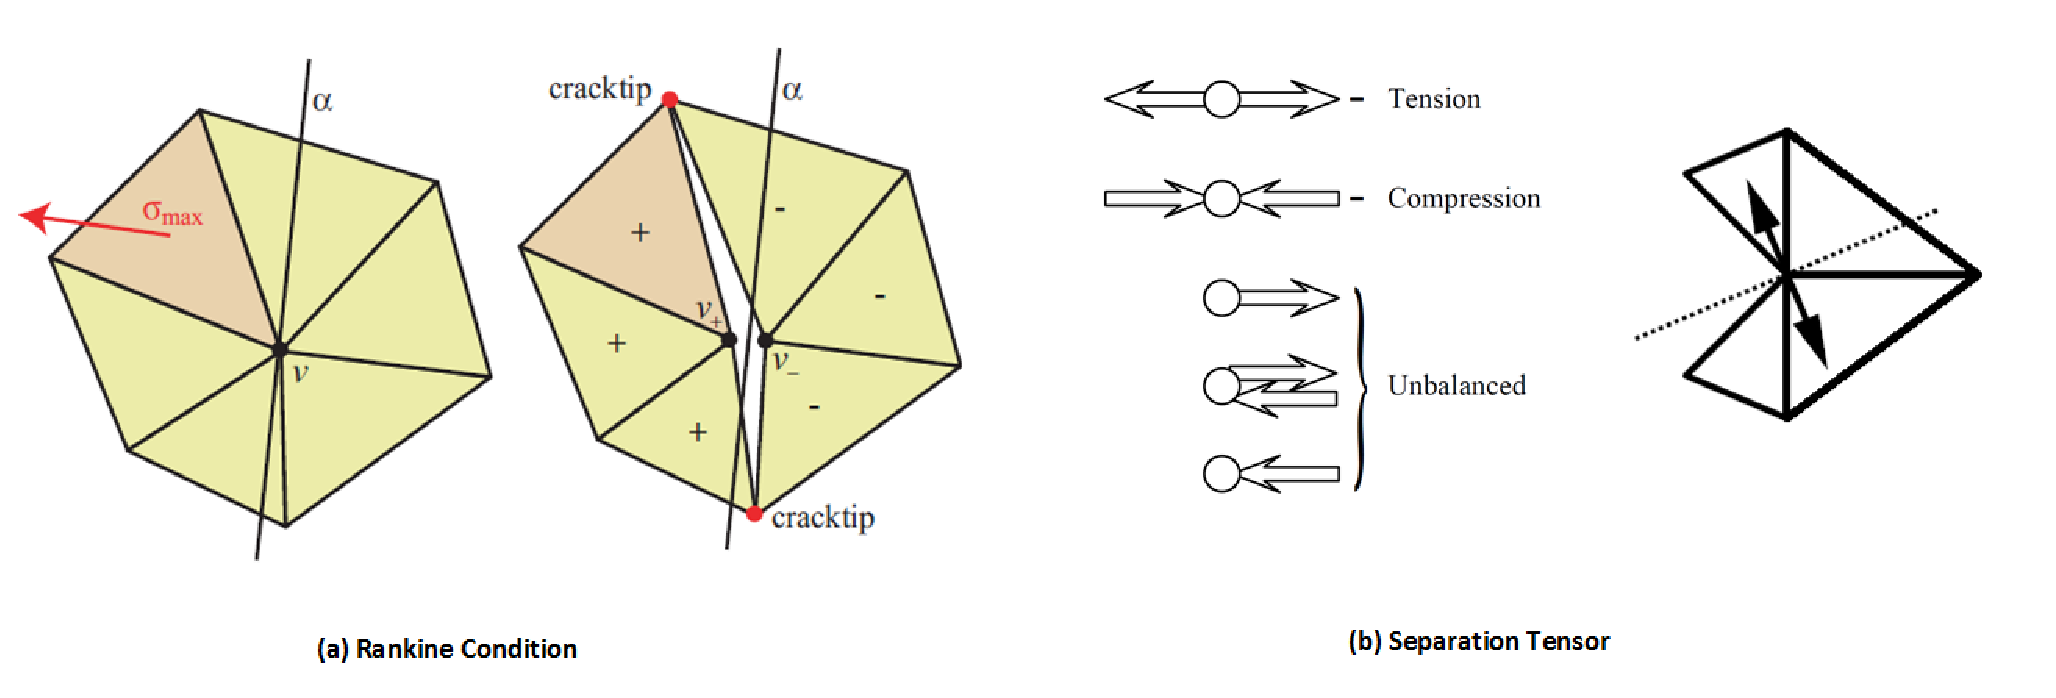
\includegraphics[width=\linewidth]{E:/Thesis-Master/chap/image/fracture_model}

  \caption{\label{fracture_model}
           碎裂模型示意图。左边为Rankine Condition,右边为 Separation Tensor。图片分别取自\textcolor{blue}{(M\"{u}ller et al. )\parencite{Muller2004}} 和\textcolor{blue}{(O'Brien et al. )\parencite{OBrien1999}}。
          }
\end{figure}

最常用的碎裂模型包括 Rankine Condition,其基本原理是计算物质节点的主应力大小$\mathbf{\sigma}_{max}$ 以及主应力方向 $\textbf{n}_{max}$,如果$\mathbf{\sigma}_{max}$ 超出阈值则认定碎裂发生,并且裂纹方向即为$\textbf{n}_{max}$。 应用此碎裂模型的典型工作包括\textcolor{blue}{(M\"{u}ller et al.)\parencite{Muller2004}}。 但Rankine Condition 的缺陷是即使某一方向受力较大,也会导致碎裂发生,而事实上碎裂是由相互抵消的力(挤压或者撕扯)的大小而决定的。因此,另一种常用的碎裂模型是 Separation Tensor\textcolor{blue}{(O'Brien et al.)\parencite{OBrien1999}} ,其计算的是相互抵消的力最大的方向和应力大小,因此克服Rankine Condition的缺陷,不过其在计算上相对要较为复杂。两种碎裂模型的示意图如图\ref{fracture_model}所示。

对于质点弹簧系统或者无网格中的方法,其拓扑关系通过粒子与粒子之间的连接而决定的。因此,在碎裂模型上往往不涉及裂纹生长的方向,而是可以直接通过去除粒子之间的相互作用力来体现。在无网格框架中,最常用的碎裂模型是临界伸长量(critical stretch)。假设粒子之间通过弹簧相连,如果其伸长比例超过阈值,则断裂发生。本文所用的碎裂模型类似于 critical stretch,但对其有所改进,具体在第三章详述。

\section{离散时间积分}
\label{numerical_method}
在章节\ref{related_work}所阐述的有网格方法和无网格方法本质上是在空间上对物体进行离散化,而求解物体的运动还需要在时间维度上进行离散化,在时间维度上的离散化数值积分被称为离散时间积分。精确性(accuracy)和稳定性(stability)是衡量离散时间积分算法优劣的两大指标,其中精确性衡量的是离散积分的解与连续解之间的误差,而稳定性衡量的是误差是否会随时间累积。关于数值积分的详细介绍,参见\mycite{Michael}{1997}。

离散时间积分决定以何种方式来对系统中的状态进行更新。在大多数系统中,通常需要关心的状态更新是位置 $\textbf{x}$ 和速度 $\textbf{v}$。 对于无网格方法,$\textbf{x}$ 和 $\textbf{v}$ 被直接赋予到粒子之上。而对于有网格方法,虽然整体的物理动力学计算是基于网格中的单元体的,但实际上单元体在拓扑上仍然由节点连接而成,最后的计算结果仍然将会以加权平均的方式施加到各个顶点。

假设某粒子 $i$ 所受内力为 $\fin$,所受外力为$\fex$,速度为$\vi$,位置为$\xii$,质量为 $m_i$。则根据速度的定义以及牛顿第二定律,得到:
\begin{equation}
\label{eq1}
\left\{ \begin{array}{l}
\frac{\textrm{d}\xii}{\textrm{d}t} = \dot{\xii}=\vi\\
\frac{\textrm{d}\dot{\xii}}{\textrm{d}t} = \frac{\textrm{d}\vi}{\textrm{d}t}=\frac{\fin + \fex}{m_i}
\end{array} \right.
\end{equation}
注意在上述公式中$\xii$和$\vi$都是关于时间的函数,离散时间积分是通过$\xii(t_0)$和$\vi(t_0)$来求解$\xii(t_0 + \Delta t)$ 和$\vi(t_0 + \Delta t)$的状态。

最常见的两种时间积分算法分别是显式欧拉积分(explicit Euler integration)和隐式欧拉积分(implicit Euler integration)。在下面小节中,我们将分别进行介绍。

\subsection{显式欧拉积分}

\begin{figure}[!htb]
  \centering
  \captionsetup{justification=centering}
  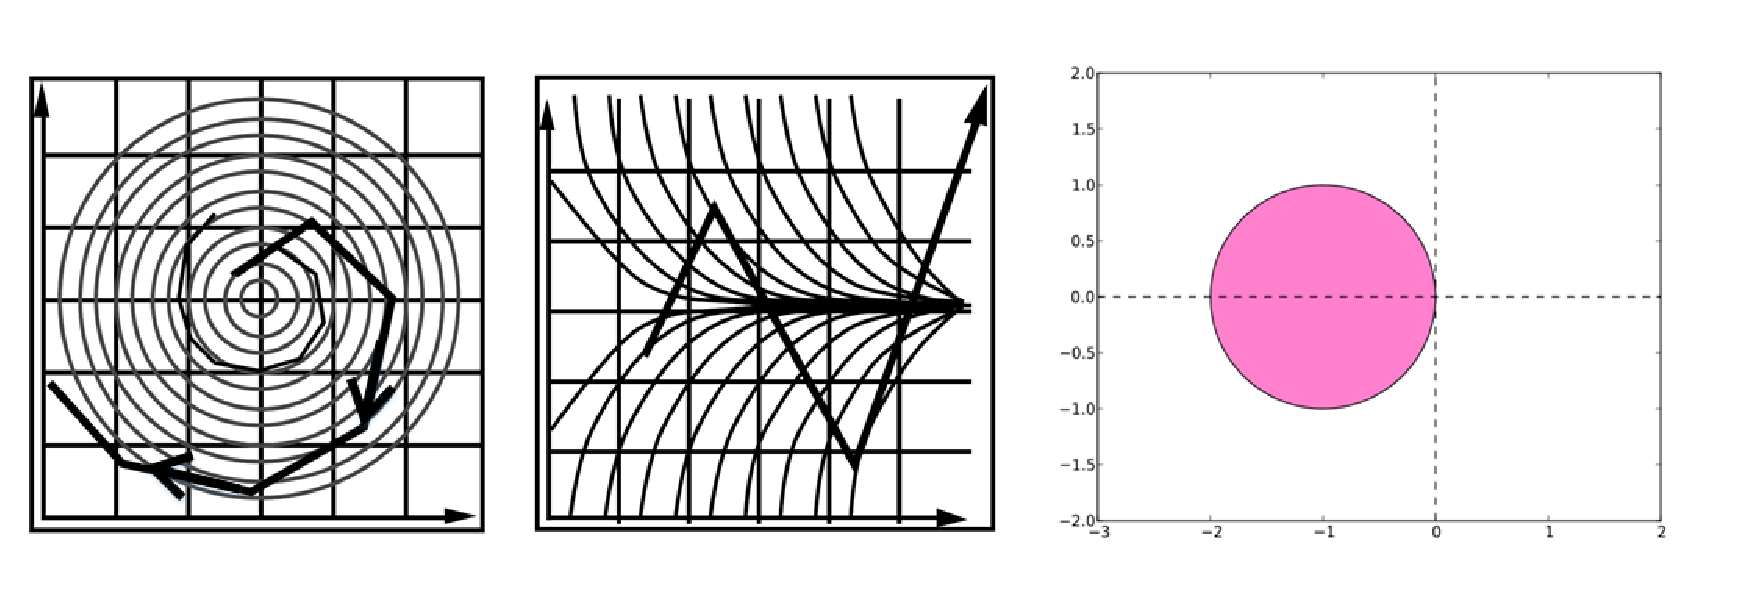
\includegraphics[width=\linewidth]{E:/Thesis-Master/chap/image/explicit_method}

  \caption{\label{explicit_method}
           显示欧拉积分。随着仿真的进行,误差将很容易累积,从而导致仿真系统崩溃。粉色区域为绝对稳定区域。图片取自\mycite{Witkin}{1997}
          }
\end{figure}

显式积分亦称前向欧拉积分(forward Euler method),其思想来源于在 $t_0$ 时刻的一阶泰勒展开 $f(t_0 + \Delta t) \approx f(t_0) + \dot{f}(t_0)\Delta t$,$t_0 + \Delta t$ 时刻的状态完全直接由 $t_0$ 时刻的状态决定。具体而言,
\begin{equation}
\left\{ \begin{array}{l}
\vi(t_0+\Delta t) = \vi(t_0)+\frac{\fin(t_0) + \fex(t_0)}{m_i}\Delta t\\
\xii(t_0+\Delta t) = \xii(t_0)+\vi(t_0)\Delta t
\end{array} \right.
\end{equation}

显式欧拉积分是最容易实现的离散积分方式,并且可以直接并行化。在数值准确性上其具备一阶数值精度,但稳定性较差。当时间步长 $\Delta t$ 较长时,容易累积误差而致使整个仿真系统崩溃,如图\ref{explicit_method}。因此使用显式积分的仿真系统往往需要设置较小的时间步,并且同时添加阻尼力保证仿真的稳定性。可以进行些许修改从而一定程度上改善其稳定性:
\begin{equation}
\left\{ \begin{array}{l}
\vi(t_0+\Delta t) = \vi(t_0)+\frac{\fin(t_0) + \fex(t_0)}{m_i}\Delta t\\
\xii(t_0+\Delta t) = \xii(t_0)+\vi(t_0 \textcolor{red}{ + \Delta t})\Delta t
\end{array} \right.
\end{equation}
这种形式的数值积分算法被称为半隐式欧拉积分(Semi-implicit Euler integration)。本文工作大部分都采用此种形式的积分算法,具体计算流程可用如下伪码表示:\\

\noindent\fbox{
\parbox{0.6\textwidth}{

//initialization\\
(1) \textbf{forall} particles $i$ \\
(2) \qquad initialize $m_i$ and other necessary info\\
(3) \qquad $\xii \leftarrow \xii(t_0)$\\
(4) \qquad $\vi \leftarrow \vi(t_0)$\\
(5) \textbf{endfor}\\\\
//simulation loop\\
(6) \textbf{loop}\\
(7) \qquad \textbf{forall} particles $i$\\
(8) \qquad \qquad calculate $\fin$ from constitutive laws\\
(8) \qquad \qquad calculate $\fex$ from boundary conditions\\
(9) \qquad \qquad $\vi\leftarrow \vi + \Delta t\cdot \frac{\fin + \fex}{m_i}$\\
(10) \qquad\qquad $\xii\leftarrow \xii +\Delta t\cdot \vi$\\
(11) \qquad\textbf{endfor}\\
(12) \qquad display the system every $n^{th}$ time\\
(13) \textbf{endloop}                   
} 
}\\

\subsection{隐式欧拉积分}
\begin{figure}[!htb]
  \centering
  \captionsetup{justification=centering}
  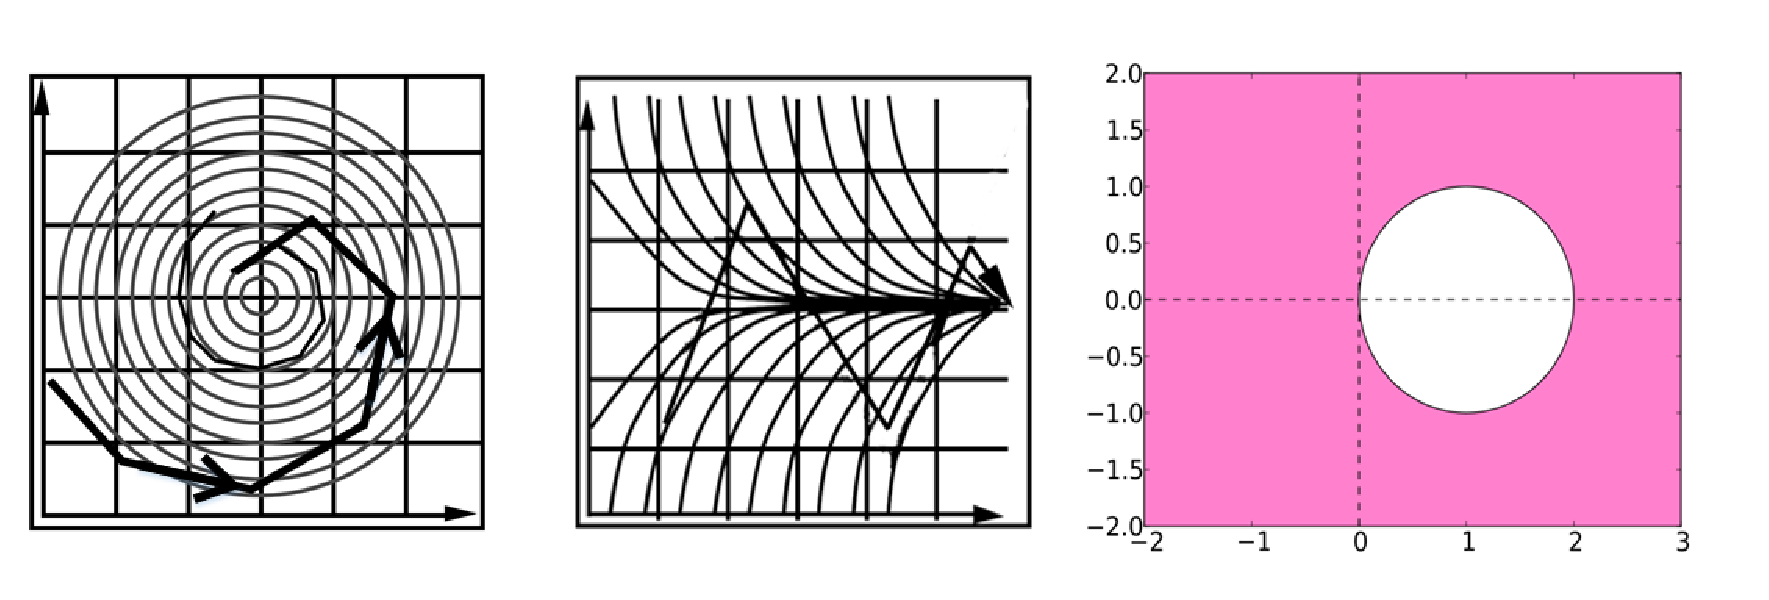
\includegraphics[width=\linewidth]{E:/Thesis-Master/chap/image/implicit_method}

  \caption{\label{implicit_method}
           隐式欧拉积分。隐式欧拉积分理论上可认为是无条件稳定的,并且自带阻尼效果。图中粉色区域为所示绝对稳定区域。
          }
\end{figure}

不同于显式欧拉积分,隐式欧拉积分理论上可认为是绝对稳定的,其误差并不随时间而积累。一般认为隐式欧拉积分方法自带阻尼效果,其会导致能量的耗散,如图\ref{implicit_method}所示。隐式欧拉积分的思想来源于在 $t_0 + \Delta t$ 时刻的一阶泰勒近似$f(t_0) \approx f(t_0 + \Delta t) - \dot{f}(t_0 + \Delta t)\Delta t$,因此也称之为向后欧拉算法(backward Euler method)。其具体积分形式可写为:
\begin{equation}
\left\{ \begin{array}{l}
\vi(t_0+\Delta t) = \vi(t_0)+\frac{\fin(t_0 \textcolor{red}{+ \Delta t}) + \fex(t_0 \textcolor{red}
                                  {+ \Delta t})}{m_i}\Delta t\\
\xii(t_0+\Delta t) = \xii(t_0)+\vi(t_0 \textcolor{red}{ + \Delta t})\Delta t
\end{array} \right.
\end{equation}

进一步,
\begin{equation}
\label{eqa25}
\left\{ \begin{array}{l}
\Delta \vi = \frac{\fin(t_0 \textcolor{red}{+ \Delta t}) + \fex(t_0 \textcolor{red}
                                  {+ \Delta t})}{m_i}\Delta t\\
\Delta \xii = \left(\vi(t_0) + \Delta \vi\right)\Delta t
\end{array} \right.
\end{equation}

其中 $\Delta \vi = \vi(t_0 + \Delta t) - \vi(t_0)$ 表示速度增量, $\Delta \xii = \xii(t_0 + \Delta t) - \xii(t_0)$ 表示位置增量,$\fin(t_0 \textcolor{red}{+ \Delta t})$ 和 $\fex(t_0 \textcolor{red}{+ \Delta t})$ 分别代表在 $t_0 + \Delta t$ 时刻的内力和外力。一般而言,$\fex(t_0 \textcolor{red}{+ \Delta t})$ 可以直接用 $\fex(t_0)$ 近似,然而$\fin(t_0 \textcolor{red}{+ \Delta t})$则不然。事实上,除非 $\fin(t_0 \textcolor{red}{+ \Delta t})$ 是线性函数,亦即所仿真材料是线性材料,否则在求解时其并非已知。因此如果$\fin(t_0 \textcolor{red}{+ \Delta t})$ 是非线性函数(即非线性材料),则此时是无法对其进行精确求解的,只能对其进行一阶泰勒近似,亦即
\begin{equation}
\fin(\xii(t_0) + \Delta \xii(t_0),\vi(t_0)+\Delta \vi) = \fin(t_0) +
                                                         \sum\frac{\partial \fin(t_0)}{\partial \xj}\Delta \xj+
                                                         \sum\frac{\partial \fin(t_0)}{\partial \vj}\Delta \vj
\end{equation}

注意在 $t_0 + \Delta t$ 时刻,$\fin$ 是关于$\xii(t_0 + \Delta t)$ 和 $\vi(t_0 + \Delta t)$的函数,通常 $\fin$ 并不和速度相关,所以上式可以进一步简化为

\begin{equation}
\label{eqa27}
\fin(t_0)+ \Delta t) = \fin(t_0) +\sum\frac{\partial \fin(t_0)}{\partial \xj}\Delta \xj
\end{equation}

将式\ref{eqa27}代入\ref{eqa25},并消去 $\Delta \xii$,则可得

\begin{equation}
\Delta \vi = \frac{\Delta t}{m_i}\left[\fin(t_0) + \fex(t_0)\right]
           + \sum\frac{\Delta t^2}{m_i} \frac{\partial \fin(t_0)}{\partial \xj}
             \left(\vj(t_0) + \Delta \vj\right)
\end{equation}

可以看出,上述公式左边是关于粒子 $i$ 的速度增量$\Delta \vi$,而右边则和周围粒子$j$的速度增量 $\Delta \vj$相关,这是由本构模型决定的。所以不同于显式方法,隐式积分方法是没有办法对状态进行单独求解的,而只能进行全局求解。我们需要将其扩充为向量形式,如下

\begin{equation}
\Delta \textbf{v} = M^{-1}\Delta t\left[\textbf{f}^{int}(t_0) + \textbf{f}^{ext}(t_0)\right]
                  + M^{-1}\Delta t^2 \frac{\partial \textbf{f}^{int}(t_0)}{\partial \textbf{x}}
                    \left(\textbf{v}(t_0) + \Delta\textbf{v}\right)
\end{equation}

其中$M$为质量对角矩阵。将上述方程进行重整,可以得到最终形式:

\begin{equation}
\left(\hat{I} - M^{-1}\Delta t^2 \frac{\partial \textbf{f}^{int}(t_0)}{\partial \textbf{x}}\right)\Delta \textbf{v} = M^{-1}\Delta t\left[\textbf{f}^{int}(t_0) + \textbf{f}^{ext}(t_0)\right]
                  + M^{-1}\Delta t^2 \frac{\partial \textbf{f}^{int}(t_0)}{\partial \textbf{x}}\textbf{v}(t_0)
\end{equation}

或

\begin{equation}
\left(M - \Delta t^2 \frac{\partial \textbf{f}^{int}(t_0)}{\partial \textbf{x}}\right)\textbf{v}(t_0 + \Delta t) = \Delta t\left[\textbf{f}^{int}(t_0) + \textbf{f}^{ext}(t_0)\right]
                  + M\textbf{v}(t_0)
\end{equation}

其中 $\textbf{K} = \frac{\partial \textbf{f}^{int}(t_0)}{\partial \textbf{x}}$ 被定义为刚度矩阵(stiffness matrix)。不难看出,在隐式积分算法下,问题最终转化为一个线性系统$\textbf{Ax} = \textbf{b}$问题的求解。对于大规模的线性矩阵求解问题,一般采用迭代法进行求解,如 Jacobi 迭代法或者 Gauss-Seidel 迭代法。其中 Jacobi 迭代法收敛速度较慢,但适于并行,Gauss-Seidel 迭代法则相反。此外,考虑刚度矩阵 $\textbf{K}$ 一般具有对称性,更多的是采用预置共轭梯度的办法来进行求解(PCG),其具有非常良好的收敛速度。在具体实现时,刚度矩阵 $\textbf{K}$ 往往不需要显式构造,只需要提供计算 $\textbf{K} \cdot \Delta \textbf{x}$ 的接口,进一步减少存储空间和提高效率。

隐式欧拉积分在 FEM 和其他无网格方法应用都较为普遍,其相对于显式积分方法在稳定性上具有明显优势。虽然隐式方法实现更为复杂,但由于能够对时间步 $\Delta t$的限制有所放松,所以最终仿真效率能够领先于显式积分方法。不过由于近场动力学本身的特殊性,其在计算刚度矩阵时$\textbf{K}$相对于一般系统要多出一层复杂度,所以在本工作中,我们只针对规模较小系统尝试隐式欧拉积分,具体原因将在第三章进行说明。




	\appendix
	\printbibliography[heading = bibintoc]

	\backmatter
	\chapter{致谢}
感谢我的导师李胜副教授。李老师是我从天体物理转向计算机图形学方向的领路人,无论是在学术上还是人生道路上,都给予了我很大帮助。感谢汪国平教授,其工作态度永远值得我们学习。

感谢朱飞师兄,没有朱飞师兄在我科研路上的不断督促和指导,以及对本工作的不断完善,本工作将是错漏百出、举步维艰的。感谢何小伟师兄、杨升师兄、徐力有师弟、朱奎鑫师弟、田然师弟在科研讨论时提供的有效思路及帮助。

感谢北京大学,从本科到硕士,度过了我最为美好、最为充实的七年时光。

最后,感谢那些还陪伴在我身边的人以及未来会陪伴在我身边的人,你们的存在是我不断努力、奋勇向前的最大动力与意义。

人生但苦无妨。未来,愿付出所有,换前所未有。


	\include{chap/originauth}

\end{document}
